\documentclass[defense.tex]{subfiles}
\begin{document}

\section{Time Series Representations}


\begin{frame}{Time series representation}
\Large

	{\bf Finding a good representation is challenging:}\\[.5em]
	\begin{itemize}\itemindent2em\itemsep.25em
		\item Samples with various lengths and scales, \\[.25em]
		\keypoint{Invariant}
		\item Heterogeneous sampling rates across channels, \\[.25em]
		\keypoint{Nonparametric}
		\item Samples have high dimension, \\[.25em]
		\keypoint{Scalable}
		\item Non stationary signals. \\[.25em]
		\keypoint{Robust}
	\end{itemize}

\end{frame}



\begin{frame}{Temporal representation}
\large
	\begin{center}
		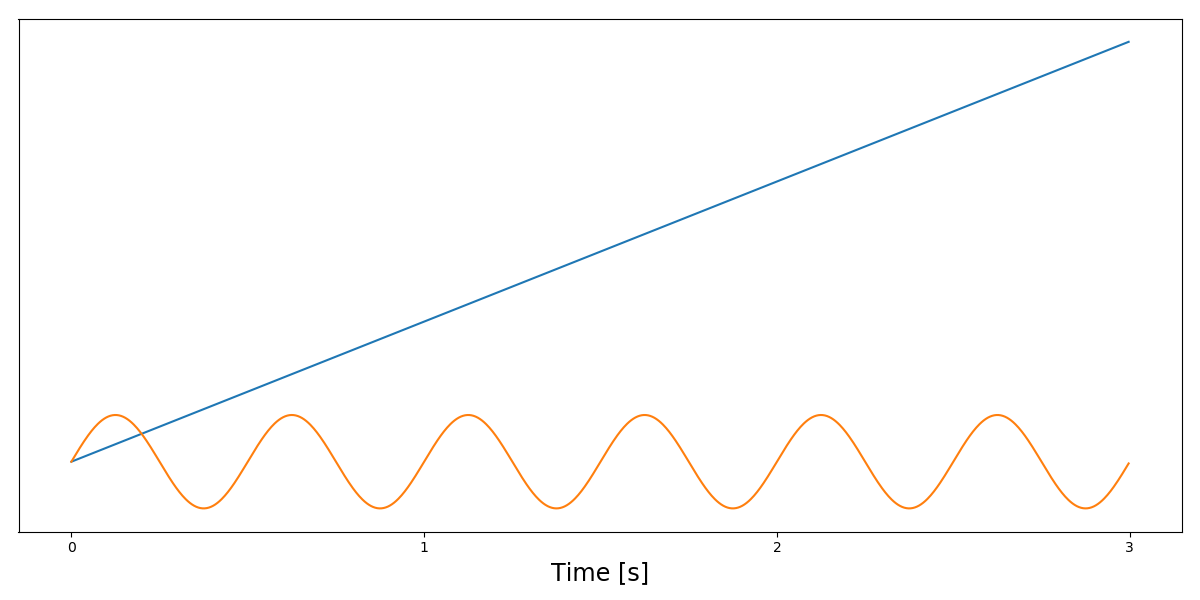
\includegraphics[width=.9\textwidth]{temporal}
	\end{center}
	\begin{itemize}\itemsep1em
		\item Most common representation \hskip1em {\usebeamercolor[fg]{itemize item}\raisebox{0.12ex}{$\blacktriangleright$}\hskip0.1em} Can be efficient (cardiologist)
		\item Permits to detect patterns (linearity, periodicity, ...)
	\end{itemize}
\end{frame}



\begin{frame}{Temporal representation}
	\begin{columns}[c]
		\column{.02\textwidth}
		\column{.5\textwidth}
		\includegraphics[width=.87\textwidth, trim={0 0 21.5em 0}, clip]{fourier_rpz}
		\column{.39\textwidth}
		{\large
		\begin{itemize}\itemsep2em
			\item Not robust to noise
			\item Limited interpretation
		\end{itemize}
		}
	\end{columns}
	
\end{frame}

\begin{frame}{Fourier representation}
	\begin{center}
		%\includegraphics[width=.87\textwidth]{fourier_rpz}
        \begin{tikzpicture}
            \node[anchor=south west,inner sep=0] (image) at (0,0) {\includegraphics[width=.87\textwidth]{fourier_rpz}};
            \node[align=center,font={\Large\bfseries}, rotate=90, above] at (image.west) {Temporal};
            \node[align=center,font={\Large\bfseries}, rotate=-90, above] at (image.east) {Fourier};
        \end{tikzpicture}
	\end{center}
	
\end{frame}



\begin{frame}{Studying the local structure}

	\centering
	{\Large Not so efficient for non stationary signals.\\[1em]}
	\begin{center}
		
        \begin{tikzpicture}
            \node[anchor=south west,inner sep=0] (image) at (0,0) {
            	\includegraphics[width=.87\textwidth, trim={0 15.7em 0 0}, clip]{stft}};
            \node[align=center,font={\Large\bfseries}, rotate=90, above] at (image.west) {Temporal};
            \node[align=center,font={\Large\bfseries}, rotate=-90, above] at (image.east) {Fourier};
        \end{tikzpicture}
	\end{center}

\end{frame}

\begin{frame}{Studying the local structure}

	\centering
	{\Large Need some time-frequency insights.\\[1em]}
	\begin{center}
		\includegraphics[width=.87\textwidth, trim={0 0 0 15.8em}, clip]{stft}
	\end{center}
	
	\Large {\bf Main idea:}\\
	apply global representation to windowed signals

\end{frame}



\begin{frame}{Analytical property}

	\centering \Large
	{\bf Main drawback: }\\[1em]
	We need to know the property we are looking for.\\[2em]
	
	Data-driven representation

\end{frame}

\end{document}